%%% Tahoe Schrader
%%% Computational Physics
%%% Spring, 2017

%%%%%%%%%%%%%%%%%%%%%%%%%%%%%%%%%%%%%%%%%%%%%%%%%%%%%%%%%%%%%%%%%%%%%%%%%%%%%%%
%%% This code will develop a LaTeX'd writeup of the Ising Model Final
%%%%%%%%%%%%%%%%%%%%%%%%%%%%%%%%%%%%%%%%%%%%%%%%%%%%%%%%%%%%%%%%%%%%%%%%%%%%%%%%

% PACKAGES AND OTHER DOCUMENT CONFIGURATIONS
\documentclass[12pt]{article}
\usepackage[english]{babel}
\usepackage[utf8]{inputenc}
\usepackage{amsmath,amsfonts,amssymb}
\usepackage{graphicx,xcolor}
\usepackage{subfig}
\usepackage{booktabs,hyperref}
\usepackage[left=2cm,%
right=2cm,%
top=2cm,%
bottom=2cm,%
headheight=11pt,%
letterpaper]{geometry}%
\usepackage{fancyhdr}
\pagestyle{fancy}
\lhead{\small\sffamily\bfseries\leftmark}%
\chead{}%
\rhead{\small\sffamily\bfseries\rightmark}
\renewcommand{\headrulewidth}{1pt}
\renewcommand{\footrulewidth}{1pt}
\graphicspath{{images/},}

% Article Information
\title{Computationally Solving the $2D$ Ising Model with the Metropolis Algorithm}
\author{Tahoe Schrader\\PHYS566}
\date{}

% Begin writing document
\begin{document}
\maketitle

% Start with the abstract

\abstract{In this paper I depict the results of computationally exploring the $2D$ Ising Model for various lattices with an interaction strength of $J=1.5$ and the Boltzmann constant set to one, solely using Python. Each lattice was cooled from $T=5\to 0$. For $n=50$, the magnetization as a function of temperature was plotted to determine a critical temperature of $T_c = 2.65$. For $n=[5, 10, 20, 30, 40, 50, 75, 100, 200, 500]$, the maximum specific heat per lattice size as a function of temperature was plotted to determine the finite-size scaling relation, $C_{\text{max}}/N \approx \log(n)$. The data matches the theory for magnetization measurements and specific heat. Nonetheless, the finite-size scaling relation, $C_{\text{max}}/N\approx \log(n)$, does not fit perfectly for either large or small $n$.}

\section{Theory}
\label{sec:theory}
The Ising model is one of the few models of a system with a phase transition that can be treated analytically. In 1925, it was introduced to describe the phase transitions of ferromagnets at the curie temperature. Nowadays, it is used to describe much physical phenomena, such as order-disorder transitions in binary alloys, spin glass, and certain neural network classes.

Lattices that obey the Ising model have periodic boundary conditions. In $1D$ and $2D$, the lattice resembles a circle or toroid, respectively. The Hamiltonian takes the form:
\begin{equation}
  \label{eq:basichamiltonian}
  H_N(\sigma_1,\ldots,\sigma_N) = -J \sum_{\text{n.n}} \sigma_i\sigma_k - \mu B\sum_{i=1}^N\sigma_i,
\end{equation}
where $\mu$ is the magnetic moment, $\sigma$ is spin up or down, $N=n^2$ is the dimension of the lattice, $J$ is the interaction strength, and $\text{n.n}$ refers to a sum across nearest neighbors. I have chosen to study the case with no external magnetic field, which causes the second term in Equation~\ref{eq:basichamiltonian} to fall out. From now on, I will refer to the Hamiltonian as the energy of the system.

\subsection{Specific Heat and Magnetization}
\label{sec:solvingforparameters}
The energy of the system is important because a large number of parameters can be solved for once the energy is obtained. An in-depth derivation of these parameters can be found in any statistical mechanics textbook. The important thing to note here is that by obtaining the partition function from the energy, the free energy can be derived. The free energy can then be manipulated to derive any thermodynamic property.

The thermodynamic property studied in this paper is specific heat. Specific heat is given by the equation:
\begin{equation}
  \label{eq:specificheat}
  C = \frac{\left(\Delta E\right)^2}{k_B T^2},
\end{equation}
where $\left(\Delta E\right)^2$ is determined computationally during a sweep through temperatures. The $\left(\Delta E\right)^2$ parameter will be discussed more thoroughly in Section~\ref{sec:determiningdE2}.

The second major property studied in this paper is the magnetization of the system. Magnetization depends on the over-arching spin alignment of the lattice. Individual spins in the lattice can have a value of $+1$ (spin up) or $-1$ (spin down). Magnetization per spin is given by,
\begin{equation}
  \label{eq:magnetizationperspin}
  M_{\text{per spin}} = \langle \sigma \rangle = \frac{1}{N}\sum_i \sigma_i,
\end{equation}
and the total magnetization is given by,
\begin{equation}
  \label{eq:magnetizationtotal}
  M_{\text{total}} = N \langle \sigma \rangle = \sum_i \sigma_i.
\end{equation}

The reason why I am focusing on specific heat and magnetization is that by juxtaposing the two against one another, a phase transition can be proven to occur. This phase transition occurs at the critical temperature, $T_c$, exhibited by a step function in magnetization and a peak in specific heat.

Lastly, the Ising model can be shown to obey a finite-size scaling relation, given by
\begin{equation}
  \label{eq:finitescaling}
  \frac{C_{\text{max}}}{N} \approx \log (n),
\end{equation}
where $n$ is simply the length of the lattice. This implies that although an infinite lattice will have an infinite specific heat, all finite lattices have a realistically measurable specific heat that scales by $N*\log(n)$. This relation is tested in Section~\ref{sec:data}.

\subsection{Determining $\left(\Delta E\right)^2$}
\label{sec:determiningdE2}
The starting point of investigating the $2D$ Ising model is a lattice of spins that can only assume two directions with respect to the $\hat{z}$-axis. These two values were described above to be $\sigma_i=\pm 1$. Energy is determined by Equation~\ref{eq:basichamiltonian} with no external field to be:
\begin{equation}
  \label{eq:energy}
  E = - J \sum_{\text{n.n}} \sigma_i\sigma_k.
\end{equation}
This sum is over all nearest neighbor pairs. Note that when computing this type of sum for a $2D$ lattice, each pair is double counted. Therefore, the nearest neighbor sum is divided by two.

Given $N_m$ total microstates, the energy expectation value is
\begin{equation}
  \label{eq:energyexpect}
  \langle E \rangle = \frac{1}{N_m}\sum_\alpha E_\alpha.
\end{equation}
The energy squared expectation value is
\begin{equation}
  \label{eq:energy2expect}
  \langle E^2 \rangle = \frac{1}{N_m}\sum_\alpha E_\alpha^2.
\end{equation}
Using Equation~\ref{eq:specificheat} with
\begin{equation}
  \label{eq:dE2}
  \left(\Delta E\right)^2 = \langle E^2\rangle-\langle E \rangle^2
\end{equation}
will then give the specific heat of the system at a given temperature.

\section{Code}
\label{sec:code}
Actually obtaining the parameters above in Python is quite difficult due to the level of randomness a heat bath adds to the system. Each individual spin in the lattice has an interaction strength of $J=1.5$. Because $J>0$, the system favors a parallel alignment of spin ($\sigma = +1$). In the absence of a heat bath, the system evolves into a fully aligned state, either spin up or down. With a heat bath, the alignment is governed by the probability
\begin{equation}
  \label{eq:probabilityheatbath}
  P_\alpha \approx e^{-E_\alpha/k_BT},
\end{equation}
where $\alpha$ is an individual microstate.

Flipping spins according to Equation~\ref{eq:probabilityheatbath} is a process known as the Metropolis Algorithm or Markov Chain analysis. The logic needed to run the Metropolis Algorithm is enumerated below:
\begin{enumerate}
  \item Initialize the system by assigning random spin orientations to each lattice point and compute the initial energy using Equation~\ref{eq:energy}.
  \item Relax system by:
  \begin{enumerate}
    \item Instigate a hypothetical spin flip at a random location, and calculate the hypothetical change in energy this flip would cause.
    \item Use the Metropolis algorithm to decide if the spin flip is kept.
    \item If kept, update the lattice and energy by adding the hypothetical change.
    \item If not kept, do not update the lattice or the energy.
    \item Repeat 2a-2d $10,000$ times.
  \end{enumerate}
  \item Measure and store $E$ and $M$. This is the first microstate.
  \item Measure and store another $N_m$ microstates of energy and magnetization by:
  \begin{enumerate}
    \item Repeat 2a-2d $100$ times. This helps give a statistically significant measurement since nearby measurements are heavily correlated.
    \item Store energy and magnetization.
    \item Repeat 4a-4b $N_m$ times. I chose $N_m=1,000$
  \end{enumerate}
  \item  Find $\langle E \rangle$, $\langle E^2\rangle, \left(\Delta E\right)^2$.
  \item Average $M$
  \item Repeat steps 2-6 for each temperature.
  \item Repeat 1-7 for each lattice size.
\end{enumerate}
This process was done for a number of different temperatures from $T=0\to 5$ for each lattice with dimensions $n = [5,10,20,30,40,50,75,100,200,500]$. The Metropolis algorithm itself says:
\begin{enumerate}
  \item If $\Delta E \leq 0$, keep the spin.
  \item If $\Delta E > 0$:
  \begin{enumerate}
    \item Pick a random number, $r$, in the range $[0,1]$.
    \item If $r \leq e^{-\Delta E/k_B T}$, keep the spin.
    \item Otherwise, do not keep the spin.
  \end{enumerate}
\end{enumerate}

\section{Results}
\label{sec:data}
It is expected that at a high initial temperature, the magnetization of a system is at around zero. After cooling the lattice down, the magnetization should fully align to $M = n^2$. Note that plotting $\frac{\mid M \mid}{N}$, instead, will show the spins to fully align at $+1$ and remove some noise. Noise is removed because there is a degeneracy in the magnetization measurements near $T_c$. This degeneracy says that there is an equal probability for $M$ measurements to be negative. So, plotting the absolute value of magnetization clears up this degeneracy. My data for $n=50$ is given in Figure~\ref{fig:magnetization}.
\begin{figure}[!htb]
\centerline{\minipage{.8\textwidth}
  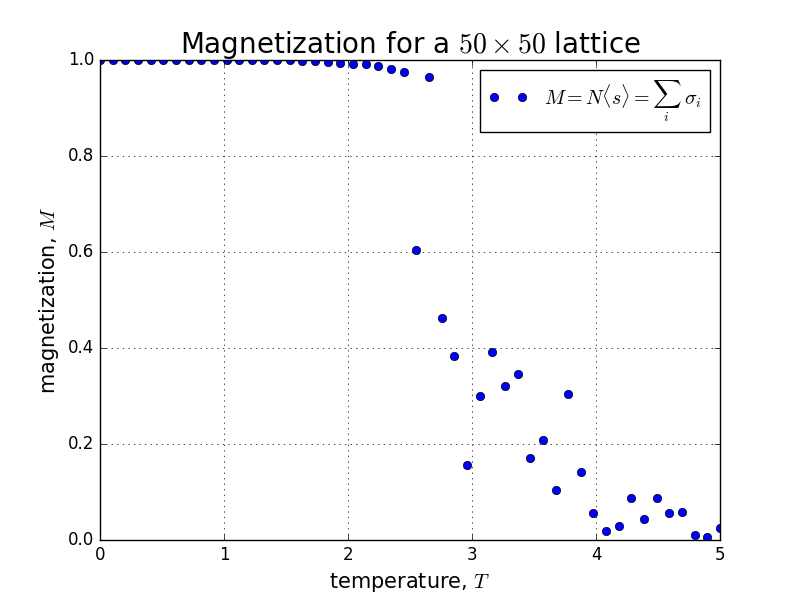
\includegraphics[width=\linewidth]{magnetization_n50.png}
  \caption{The magnetization of a $2D$ system, divided by $N$, as a function of temperature. At $T=5$, the magnetization is zero. At $T=0$, it is near $1$. The critical temperature, $T_c=2.65$, is found by noting the location of the step function at $M=0.5$, by eye.}\label{fig:magnetization}
  \endminipage}
\end{figure}

When a lower temperature resolution is used, the data becomes much worse. This can be seen in Figure~\ref{fig:worsemagnetization}. I used this temperature resolution for the rest of my calculations, which may explain some slight deviations from what is expected from the theory. 
\begin{figure}[!htb]
\centerline{\minipage{.6\textwidth}
  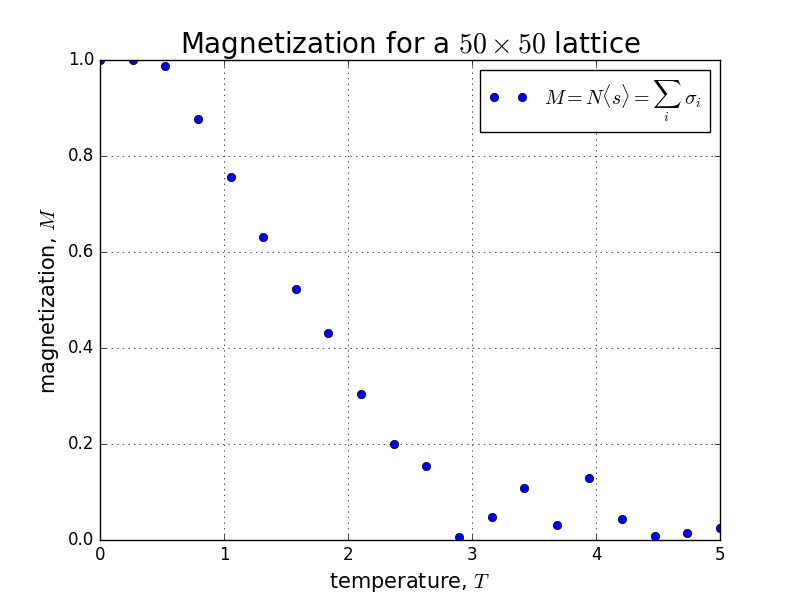
\includegraphics[width=\linewidth]{magnetization_n50_fewT.png}
  \caption{The magnetization of a $2D$ system, divided by $N$, as a function of temperature. At $T=5$, the magnetization is zero. At $T=0$, it is near $1$. Due to the low temperature resolution, the results are much worse than those displayed in Figure~\ref{fig:magnetization}}\label{fig:worsemagnetization}
  \endminipage}
\end{figure}\newpage

The specific heat for each lattice is expected to resemble a curve with a peak near its critical temperature. This peak location is called $C_{\text{max}}$. A couple example plots of specific heat are given in Figures~\ref{fig:specificheatn5}-\ref{fig:specificheatn20}.
\begin{figure}[!htb]
\minipage{0.3\textwidth}
  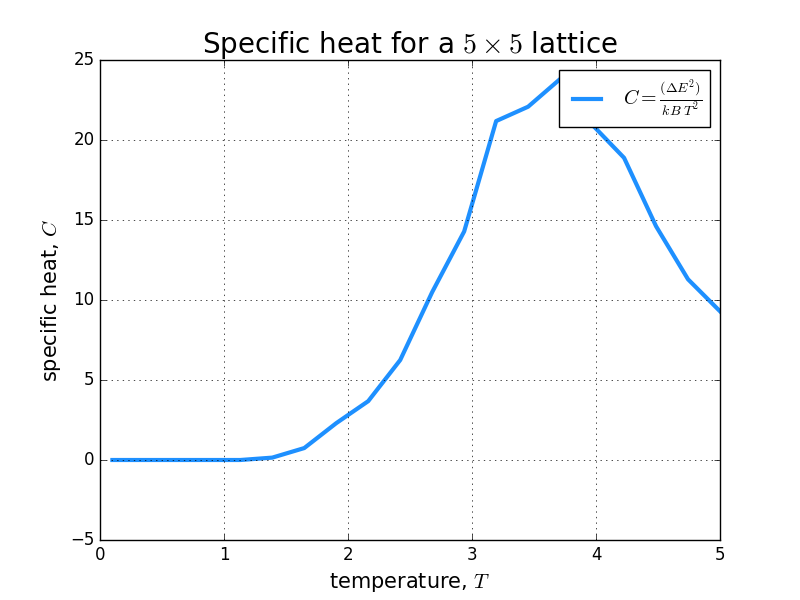
\includegraphics[width=\linewidth]{specificheat_n5.png}
  \caption{$C$ as a function of $T$ for $n=5$.}\label{fig:specificheatn5}
\endminipage\hfill
\minipage{0.3\textwidth}
  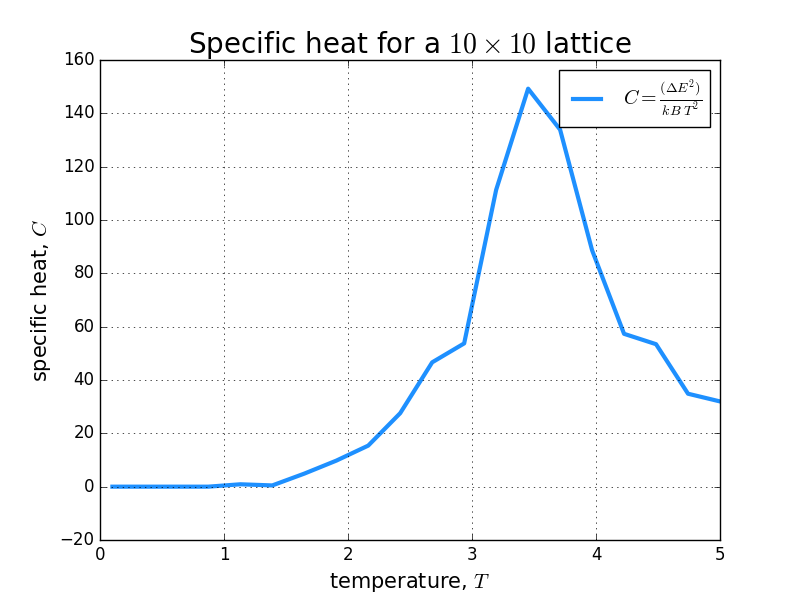
\includegraphics[width=\linewidth]{specificheat_n10.png}
  \caption{$C$ as a function of $T$ for $n=10$.}\label{fig:specificheatn10}
\endminipage\hfill
\minipage{0.3\textwidth}
  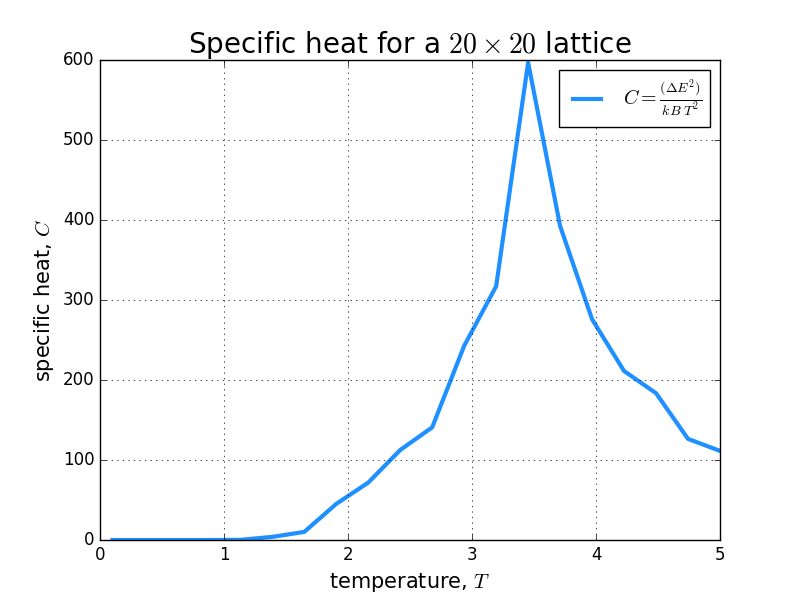
\includegraphics[width=\linewidth]{specificheat_n20.png}
  \caption{$C$ as a function of $T$ for $n=20$.}\label{fig:specificheatn20}
\endminipage\hfill
\end{figure}

Lastly, the maximum of each specific heat function was obtained and divided by $N$ in order to obtain the finite-size scaling relation. A plot of this relation is given in Figure~\ref{fig:scalingrelation}. The fit does not work well for large values of $n$. One possible reason for this is that larger values of $n$ need a longer relaxation time. This may be because the code sees the lattice as ``infinite'' with the given relaxation time of $10,000$ flips. Due to time constraints, I was not able to run the code for a longer relaxation time in order to test this. The data could have also been improved by using a finer temperature resolution. Again, due to time constraints, I was only able to solve for specific heat across $20$ temperatures from $T=5\to 0$.
\begin{figure}[!htb]
\centerline{\minipage{.6\textwidth}
  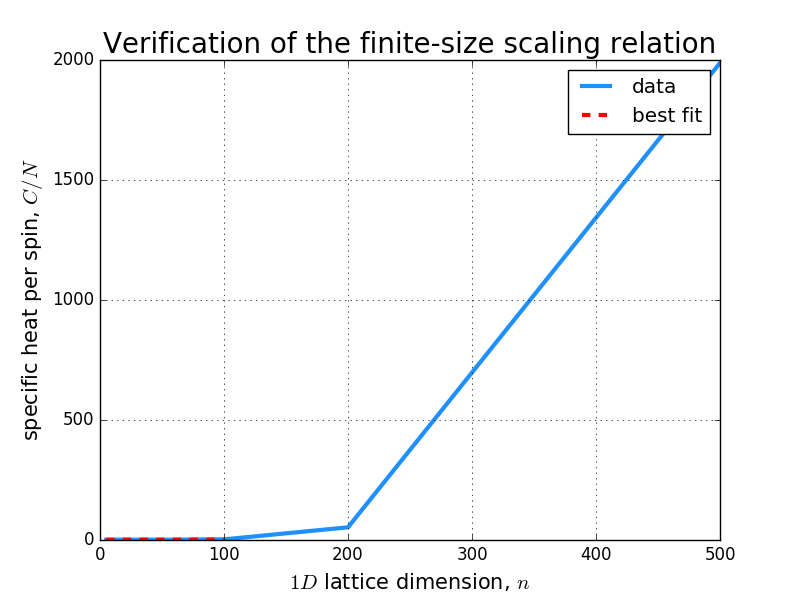
\includegraphics[width=\linewidth]{scaling_relation_zoomout.png}
  \caption{The scaling relation for $C_{\text{max}}/ N$ is depicted for $n = [5,10,20,30,40,50,75,100,200,500]$. The data should resemble $\log (n)$, as determined by a fit, but it clearly does not for large values of $n$.}\label{fig:scalingrelation}
  \endminipage}
\end{figure}

Zooming in to Figure~\ref{fig:scalingrelation}, shows what the data looks like for small $n$. These results are shown in Figures~\ref{fig:scalingrelation2} and \ref{fig:scalingrelation3}.
\begin{figure}[!htb]
\minipage{0.45\textwidth}
  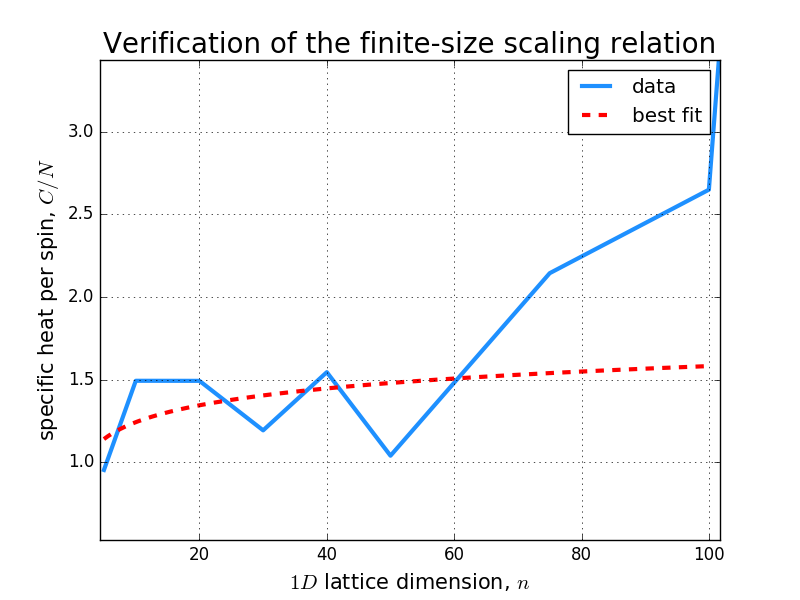
\includegraphics[width=\linewidth]{scaling_relation_zoomin.png}
  \caption{The scaling relation for $C_{\text{max}}/ N$ is depicted for $n = [5,10,20,30,40,50,75,100]$. The line of best-fit does not match the data very well. A number of different factors could have caused this, such as a low relaxation time and low temperature resolution.}\label{fig:scalingrelation2}
\endminipage\hfill
\minipage{0.45\textwidth}
  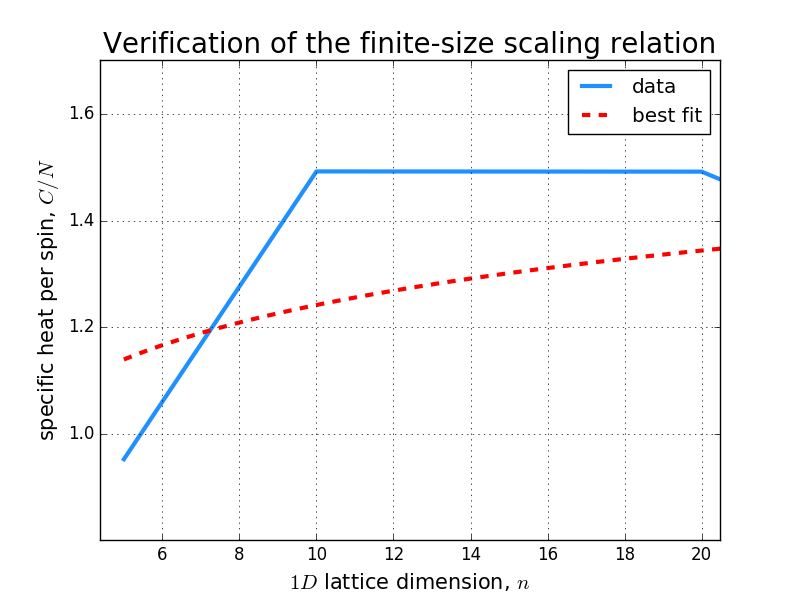
\includegraphics[width=\linewidth]{scaling_relation_smallN.png}
  \caption{The scaling relation for $C_{\text{max}}/ N$ is depicted for $n = [5,10,20]$. The line of best-fit does not match the data very well, because it includes $n=[30,40,50,75,100]$, which skewed the results. Due to time constraints, I was not able to refit the results for fewer data points.}\label{fig:scalingrelation3}
\endminipage\hfill
\end{figure}


\end{document}
